% introduccion.tex
%
% Describe el objetivo, alcance y contenido del documento.
%
%---------------------------------------------------------

%=========================================================
%---------------------------------------------------------
\chapter{Diagramas BPMN}
\label{chapter:bpmn}

	Los diagramas BPMN\footnote{Notación para el Modelado de Procesos de Negocio o BPMN por sus siglas en Inglés (Business Process Modeling Notation).} son una notación gráfica estandarizada que permite el modelado de procesos de negocio en un formato de flujo de trabajo. El objetivo es proporcionar una notación estándar que sea fácilmente legible y entendible por parte de todos los involucrados e interesados del negocio.\\

	Los diagramas BPMN, a diferencia de los diagramas de flujo, permiten modelar el flujo de información entre diversas áreas y organizaciones, el tiempo que toma realizar cierta tarea y los productos generados. Por lo que se determinó la conveniencia de modelar el proceso del CALMÉCAC a través de este estándar.

%\noindent Los diagramas BPMN tienen la característica de mostrar la interacción existente entre las diferentes áreas, entidades o actores de la organización, esto permite visualizar el flujo de la información a través de las áreas.\\

%---------------------------------------------------------
\section{Procesos, Subprocesos y Tareas}

{\bf Proceso.} Es una serie de actividades (coordinadas u organizadas) bien definidas, que se realizan (alternativa o simultáneamente) bajo ciertas circunstancias con un fin determinado. Un proceso puede involucrar: ninguno o más de un {\bf subproceso} y una o varias {\bf tareas}.\\
% 	\begin{figure}[!h]
% 	\centering\noindent{
\includegraphics[width=225pt]{introduccion/imagenes/procesos/bpmn/CollapsedSubprocess.png}}%
% 	\caption{Diagrama de un proceso.}
% 	\label{Intro:CollapsedSubprocess}
% 	\end{figure}

{\bf Subproceso.} Es muy similar al {\bf proceso}, con la única diferencia de que éste sólo puede existir o suceder dentro de un proceso. Está representado por la Figura \ref{Intro:iProceso}.\\
 	\begin{figure}[!h]
 	\centering\noindent{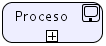
\includegraphics[width=71pt]{introduccion/imagenes/procesos/SubProceso}}%
 	\caption{Representación de un Proceso y/o Subproceso.}
 	\label{Intro:iProceso}
 	\end{figure}
% 	\begin{figure}[!h]
% 	\centering\noindent{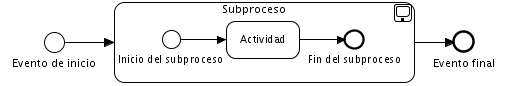
\includegraphics[width=360pt]{introduccion/imagenes/procesos/bpmn/ExpandedSubprocess.png}}%
% 	\caption{Diagrama de un subproceso expandido.}
% 	\label{Intro:ExpandedSubprocess}
% 	\end{figure}

{\bf Tarea o Actividad.} Es el grado de especificación más simple de un proceso (i.e; es el máximo detalle al que puede llegar un proceso) y de ella no pueden derivar más subprocesos o tareas. Está representado por la Figura \ref{Intro:iTarea}.
 	\begin{figure}[!h]
 	\centering\noindent{
\includegraphics[width=68pt]{introduccion/imagenes/procesos/Tarea}}%
 	\caption{Representación de una Tarea.}
 	\label{Intro:iTarea}
 	\end{figure}
% 	\begin{figure}[!h]
% 	\centering\noindent{
\includegraphics[width=240pt]{introduccion/imagenes/procesos/bpmn/SubprocessDiagram.png}}%
% 	\caption{Diagrama de un subproceso colapsado.}
% 	\label{Intro:CollapsedSubprocess}
% 	\end{figure}


%---------------------------------------------------------
\section{Subprocesos expandidos y contraídos}

{\bf Subproceso expandido.} Los subprocesos en BPMN, pueden representarse como se muestra en la Figura \ref{Intro:ExpandedSubprocess}. Esto significa que un subproceso puede contener varias actividades o subprocesos ``hijos''.
	\begin{figure}[!h]
	\centering\noindent{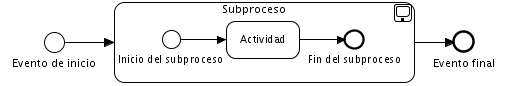
\includegraphics[width=360pt]{introduccion/imagenes/procesos/bpmn/ExpandedSubprocess.png}}%
	\caption{Subproceso expandido.}
	\label{Intro:ExpandedSubprocess}
	\end{figure}

{\bf Subproceso contraído.} Los subprocesos en BPMN, también pueden representarse como se muestra en la Figura \ref{Intro:CollapsedSubprocess}. Esta representación significa lo mismo que la Figura \ref{Intro:ExpandedSubprocess}, pero sin mostrar explícitamente sus actividades o subprocesos ``hijos''.
	\begin{figure}[!h]
	\centering\noindent{
\includegraphics[width=260pt]{introduccion/imagenes/procesos/bpmn/CollapsedSubprocess.png}}%
	\caption{Subproceso contraído.}
	\label{Intro:CollapsedSubprocess}
	\end{figure}

% {\bf Diagrama de un subproceso.} Los subprocesos en BPMN, también pueden representarse como en la Figura \ref{Intro:ExpandedCollapsed}. Esta representación significa lo mismo que la Figura \ref{Intro:ExpandedSubprocess}, pero sin mostrar explícitamente sus actividades o subprocesos ``hijos''.
% 	\begin{figure}[!h]
% 	\centering\noindent{
\includegraphics[width=360pt]{introduccion/imagenes/procesos/bpmn/SubprocessDiagram.png}}%
% 	\caption{Intro:Activity}
% 	\label{Intro:CollapsedSubprocess}
% 	\end{figure}


%---------------------------------------------------------
\section{Eventos}

Un {\bf evento} en BPMN representa algo que sucede o podría suceder durante el curso de un proceso y que afecta su flujo. Existen diferentes tipos de eventos:

\begin{itemize}
	\item {\bf Eventos iniciales}. Estos eventos inician el flujo del proceso y no tienen flujos de entrada.

	\arrayrulecolor{white}%
	\begin{tabular}{| m{.08\textwidth} m{.77\textwidth} | }% %{| c{.08\textwidth}  c{.77\textwidth} | }%
		\rowcolor[gray]{0.97}%
		\centering\noindent
\includegraphics[width=18pt]{introduccion/imagenes/procesos/bpmn/StartEvent.png} & {\bf Evento inicial simple}. No se especifica algún comportamiento en particular para empezar un proceso. \\
		\centering\noindent
\includegraphics[width=18pt]{introduccion/imagenes/procesos/bpmn/MessageEventStart.png} & {\bf Evento inicial de mensaje}. Un proceso empieza cuando un mensaje es recibido. \\
		\rowcolor[gray]{0.97}%
		\centering\noindent
\includegraphics[width=18pt]{introduccion/imagenes/procesos/bpmn/TimerEventStart.png} & {\bf Evento inicial de tiempo}. Un proceso empieza en determinada fecha o tiempo específico. \\
		\centering\noindent
\includegraphics[width=18pt]{introduccion/imagenes/procesos/bpmn/RuleEventStart.png} & {\bf Evento intermedio de regla de negocio}. Un proceso inicia cuando una condición de negocio se cumple. \\
		\rowcolor[gray]{0.97}%
		%LINK
		\centering\noindent
\includegraphics[width=18pt]{introduccion/imagenes/procesos/bpmn/LinkEventStart.png} & {\bf Evento inicial de link}. \\
		\centering\noindent
\includegraphics[width=18pt]{introduccion/imagenes/procesos/bpmn/MultipleEndEvent.png} & {\bf Evento inicial múltiple}. Indica que existen muchas formas de iniciar el proceso y que al cumplirse una de ellas se iniciará el proceso. \\
	\end{tabular}%

	\item {\bf Eventos intermedios}. Indican que algo ocurre o podría ocurrir en alguna parte del proceso (desde el inicio y hasta el final). Estos eventos pueden ser usados como parte del flujo de secuencia o adjuntarse a los bordes de una actividad para indicar que la actividad se ejecuta una vez que el evento es activado.

	\arrayrulecolor{white}%
	\begin{tabular}{| m{.08\textwidth} m{.77\textwidth} | }%
		\rowcolor[gray]{0.97}%
		\centering\noindent
\includegraphics[width=18pt]{introduccion/imagenes/procesos/bpmn/IntermediateEvent.png} & {\bf Evento intermedio sin especificar}. Indica algo que ocurre o puede ocurrir dentro del proceso, sólo se pueden utilizar dentro de la secuencia del flujo. \\
		\centering\noindent
\includegraphics[width=18pt]{introduccion/imagenes/procesos/bpmn/MessageEvent.png} & {\bf Evento intermedio de mensaje}. Indica que un mesaje puede ser enviado o recibido en alguna parte del proceso. \\
		\rowcolor[gray]{0.97}%
		\centering\noindent
\includegraphics[width=18pt]{introduccion/imagenes/procesos/bpmn/TimerEventIntermediate.png} & {\bf Evento intermedio de tiempo}. Indica que el proceso debe esperar un tiempo especifico para poder continuar.\\
		\centering\noindent
\includegraphics[width=18pt]{introduccion/imagenes/procesos/bpmn/ErrorIntermediateEvent.png} & {\bf Evento intermedio de error}. Eta figura es usada para capturar errores. Se diagrama a los límites de una actividad. \\
		\rowcolor[gray]{0.97}%
		\centering\noindent
\includegraphics[width=18pt]{introduccion/imagenes/procesos/bpmn/CancelIntermediateEvent.png} & {\bf Evento intermedio de cancelación}. Este tipo de evento intermedio es usado en subprocesos Transaccionales. Se diagrama a los límites del Subproceso transaccional indicando un flujo alternativo que se realizaría cuando el subproceso transaccional es cancelado. Se diagrma a los límites del subproceso. \\
		\centering\noindent
\includegraphics[width=18pt]{introduccion/imagenes/procesos/bpmn/CompensationIntermediateEvent.png} & {\bf Evento intermedio de compensación}. Permite manejar compensaciones. Puede ser usado dentro de la secuencia del flujo para indicar que se requiere una compensación, o adjuntado a los bordes de una actividad para indicar que la actividad será compensada una vez que el evento sea activado.\\
		\rowcolor[gray]{0.97}%
		\centering\noindent
\includegraphics[width=18pt]{introduccion/imagenes/procesos/bpmn/ConditionalIntermediateEvent.png} & {\bf Evento intermedio de condición}. Se usa cuando el flujo necesita esperar por una condición de negocio para ser completado. Sólo puede usarse dentro de la secuencia del flujo o adjuntado a los bordes de una actividad para indicar que existe un flujo de excepción. \\
		\centering\noindent
\includegraphics[width=18pt]{introduccion/imagenes/procesos/bpmn/LinkIntermediateEvent.png} & {\bf Evento intermedio de condición}. Este evento permite conectar dos secciones del proceso y puede ser usado únicamente dentro del flujo del proceso.\\
		\rowcolor[gray]{0.97}%
		\centering\noindent
\includegraphics[width=18pt]{introduccion/imagenes/procesos/bpmn/MultipleIntermediateEvent.png} & {\bf Evento intermedio múltiple}. Este evento puede ser activado por muchas causas o sólo por una de ellas. Sólo puede usarse dentro de la secuencia del flujo.\\
	\end{tabular}%

	\item {\bf Eventos finales}. Estos eventos finalizan el flujo del proceso, por lo tanto no pueden tener flujos de salida.

	\arrayrulecolor{white}%
	\begin{tabular}{| m{.08\textwidth} m{.77\textwidth} | }%
		\rowcolor[gray]{0.97}%
		\centering\noindent
\includegraphics[width=18pt]{introduccion/imagenes/procesos/bpmn/End.png} & {\bf Evento final sin especificar.} Indica que un camino del flujo llego al fin. \\
		\centering\noindent
\includegraphics[width=18pt]{introduccion/imagenes/procesos/bpmn/MessageEndEvent.png} & {\bf Evento de in de mensaje.} Permite enviar un mensaje al finalizar el flujo.\\
		\rowcolor[gray]{0.97}%
		\centering\noindent
\includegraphics[width=18pt]{introduccion/imagenes/procesos/bpmn/ErrorEndEvent.png} & {\bf Evento de fin de error.} Permite enviar una excepción de error al finalizar el flujo. \\
		\centering\noindent
\includegraphics[width=18pt]{introduccion/imagenes/procesos/bpmn/CancelEndEvent.png} & {\bf Evento final de cancelación}. Permite enviar una excepción de error cuando el flujo llega al final. Este evento solo puede usarse en subprocesos. \\
		\rowcolor[gray]{0.97}%
		\centering\noindent
\includegraphics[width=18pt]{introduccion/imagenes/procesos/bpmn/CompensationEndEvent.png} & {\bf Evento de fin de compensación.} Este tipo de fin indica que es necesaria una compensación al finalizar el flujo. \\
		\centering\noindent
\includegraphics[width=18pt]{introduccion/imagenes/procesos/bpmn/LinkEvent.png} & {\bf Evento final de liga}. Este evento permite conectar dos secciones del proceso. Sólo puede usarse dentro del flujo del proceso.\\
		\rowcolor[gray]{0.97}%
		\centering\noindent
\includegraphics[width=18pt]{introduccion/imagenes/procesos/bpmn/EndEvent.png} & {\bf Evento final.} Indica que el proceso y todas las actividades terminan, sin importar que alguna haya quedado pendiente. \\
		\centering\noindent
\includegraphics[width=18pt]{introduccion/imagenes/procesos/bpmn/MultipleEndEvent.png} & {\bf Evento de fin múltiple} Indica que varios resultados pueden darse al finalizar un flujo. \\

	\end{tabular}%
\end{itemize}

%---------------------------------------------------------
\section{Compuertas}

Las {\bf compuertas} son elementos usados para controlar la divergencia y convergencia del flujo (separar y unir).\\

	\arrayrulecolor{white}%
	\begin{tabular}{| m{.08\textwidth} m{.77\textwidth} | }%
		\rowcolor[gray]{0.97}%
		\centering\noindent
\includegraphics[width=25pt]{introduccion/imagenes/procesos/bpmn/ExclusiveGateway.png} & {\bf Compuerta exclusiva basado en los datos}. Como decisión exclusiva, tiene dos o más flujos de secuencia alternos, pero solo uno de ellos puede tomarse basado en la condición de los datos. Como convergencia, es usado para mezclar rutas alternas en una sola. \\
		\centering\noindent
\includegraphics[width=25pt]{introduccion/imagenes/procesos/bpmn/EventBasedGateway.png} & {\bf Compuerta exclusiva basada en eventos}. Representa un punto del proceso donde se escoge un camino de varios disponibles, pero la decisión no se basa en datos del proceso sino en eventos.\\
		\rowcolor[gray]{0.97}%
		\centering\noindent
\includegraphics[width=25pt]{introduccion/imagenes/procesos/bpmn/InclusiveGateway.png} & {\bf Compuerta inclusiva}. Como divergencia, es usada cuando en un punto del flujo una o más rutas puden ser activadas y la decisión está basada en los datos del proceso. Como convergencia, indica que las rutas activas son sincronizadas en una sola.\\
		\centering\noindent
\includegraphics[width=25pt]{introduccion/imagenes/procesos/bpmn/ComplexGateway.png} & {\bf Compuerta compleja}. Como divergencia, es utilizada para controlar puntos de decisión complejo. Como convergencia, permite continuar al siguiente punto del proceso cuando una condición de negocio se cumple.\\
		\rowcolor[gray]{0.97}%
		\centering\noindent
\includegraphics[width=25pt]{introduccion/imagenes/procesos/bpmn/ParallelGateway.png} & {\bf Compuerta paralela}. Como divergencia, es usada para crear rutas paralelas. Como convergencia, sincroniza multiples rutas paralelas en una. El flujo continúa cuando todas las rutas alcanzan la compuerta. \\
	\end{tabular}%

%---------------------------------------------------------
\section{Conectores}

Los {\bf conectores} son elementos usados para conectar objetos (tareas, subprocesos, eventos, compuertas, etc.) dentro del flujo.\\

	\arrayrulecolor{white}%
	\begin{tabular}{| m{.33\textwidth}  m{.52\textwidth} | }%
		\rowcolor[gray]{0.97}%
		\centering\noindent
\includegraphics[width=120pt]{introduccion/imagenes/procesos/bpmn/SequenceFlow.png} & {\bf Flujo de secuencia}. Representa el control del flujo y la secuencia de las actividades, compuertas y eventos. \\
		\centering\noindent
\includegraphics[width=120pt]{introduccion/imagenes/procesos/bpmn/MessageFlow.png} & {\bf Flujo de mensaje}. Es usado para mostrar el flujo de mensajes entre dos entidades o procesos. Representa señales o mensajes, {\bf no el control del flujo}. {\bf No todos los flujos de mensaje son secuenciales o esto especificaría orden en los mensajes}.
	\end{tabular}%


%---------------------------------------------------------
\section{Contenedores}

Un {\bf contenedor} es un elemento utilizado en BPMN para distinguir visualmente las responsabilidades entre las áreas u organizaciones.\\

	\arrayrulecolor{white}%
	\begin{tabular}{| m{.33\textwidth}  m{.52\textwidth} | }%
		\rowcolor[gray]{0.97}%
		\centering\noindent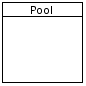
\includegraphics[width=45pt]{introduccion/imagenes/procesos/bpmn/Pool.png} & {\bf Pool}. Un {\it pool} es un contenedor representando un sólo proceso. \\%El nombre del {\it pool} puede ser considerado el nombre del proceso. \\
		\centering\noindent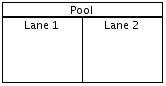
\includegraphics[width=70pt]{introduccion/imagenes/procesos/bpmn/Lane.png} & {\bf Lane}. Un {\it lane} es una subdivisión de un {\it pool} y representa un rol o área organizaquecional.
	\end{tabular}%


%- - - - - - - - - - -  - - - - - - - - - -  - - - - -

\section{Código de Colores}
\label{section:CodigoColores}

\subsection{Arquitecturas}

Para la arquitectura, los \textit{pools} horizontales representan el área o departamento encargado del proceso, los \textit{lanes} representan el proceso que se modelará.\\
El relleno(\textit{fill}) de estos elementos deberá ser \textit{Grandient Light Blue} con el 80\% de transparencia como se muestra en la figura \ref{fig:poolProceso}. Color 1 del gradiente : \textit{RGB(150,223,255)}, color 2  del gradiente: \textit{RGB(102,180,255)}.

\begin{figure}[hbtp!]
	\begin{center}
		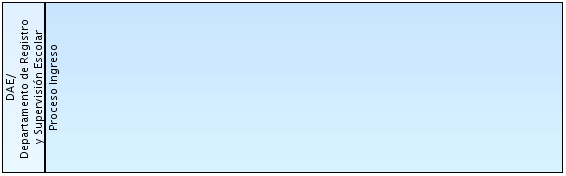
\includegraphics[width=.3\textwidth]{introduccion/imagenes/procesos/PoolProceso}
		\caption{Pool del Proceso}
		\label{fig:poolProceso}
	\end{center}
\end{figure}

Los \textit{pools} verticales representan el área o departamento externo al proceso, el \textit{lane} representa el proceso que realizan estas áreas que aporta al proceso que se desea modelar.\\
El relleno(\textit{fill}) de estos elementos deberá ser \textit{Gradient Gray} con el 80\% de transparencia como se muestra en la figura \ref{fig:poolExterno}. El color 1 del gradiente es \textit{RGB(245,245,245)} y el color 2 \textit{RGB(201,201,201)}.

\begin{figure}[hbtp!]
	\begin{center}
		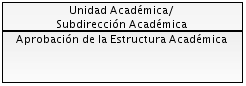
\includegraphics[width=.3\textwidth]{introduccion/imagenes/procesos/PoolExterno}
		\caption{Pool del Proceso Externo}
		\label{fig:poolExterno}
	\end{center}
\end{figure}

El \textit{pool} que se usará para representar al \refElem{Calmecac} utiliza color \textit{RGB(128,0,0)} al 80\% de transparencia como relleno(\textit{fill}) como se muestra en la figura \ref{fig:poolCalmecac}.

\begin{figure}[hbtp!]
	\begin{center}
		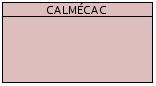
\includegraphics[width=.3\textwidth]{introduccion/imagenes/procesos/PoolCalmecac}
		\caption{Pool del Calmecac}
		\label{fig:poolCalmecac}
	\end{center}
\end{figure}

\section{Macroprocesos y Subprocesos}

Los \textit{pools} representan áreas y departamentos que están involucrados en el proceso y su relleno es \textit{Light Gray} al 80\% de transparencia si son áreas externas y completamente transparentes si son áreas que forman parte del proceso a modelar.
El \refElem{Calmecac} tendrá el mismo color como en la figura \ref{fig:poolCalmecac}.

\section{Cambios}

Para mostrar los cambios en tareas y flechas de comunicación respecto al diagrama anterior se usará una línea de color \textit{RGB(179,89,0)} con un valor de 2 en el peso y las tareas tienen el relleno(\textit{fill})  \textit{Golden} con el 80\% de transparencia como se muestra en la figura \ref{fig:TareasYFlujos}



\begin{figure}[hbtp!]
	\begin{center}
		
\includegraphics[width=.3\textwidth]{introduccion/imagenes/procesos/ArrowCambios}
		\caption{Flecha para mostrar los cambios}
		\label{fig:TareasYFlujos}
	\end{center}
\end{figure}



 







